
\documentclass{article} % For LaTeX2e
\usepackage{icais2025_conference,times}

% Optional math commands from https://github.com/goodfeli/dlbook_notation.
\input{math_commands.tex}

\usepackage{hyperref}
\hypersetup{
    colorlinks=true,
    linkcolor=blue!70!black,
    citecolor=green!60!black,
    urlcolor=red!60!black
}
\usepackage{url}

\usepackage{amsmath}
\usepackage{amssymb}
\usepackage{array}
\usepackage{algorithm}
\usepackage{algorithmicx}
\usepackage{algpseudocode}
\usepackage{booktabs}
\usepackage{colortbl}
\usepackage{color}
\usepackage{enumitem}
\usepackage{fontawesome5}
\usepackage{float}
\usepackage{graphicx}
\usepackage{hyperref}
\usepackage{listings}
\usepackage{makecell}
\usepackage{multicol}
\usepackage{multirow}
\usepackage{pgffor}
\usepackage{pifont}
\usepackage{soul}
\usepackage{sidecap}
\usepackage{subcaption}
\usepackage{tabularx}
\usepackage{titletoc}
\usepackage[symbol]{footmisc}
\usepackage{url}
\usepackage{wrapfig}
\usepackage{xcolor}
\usepackage{xspace}
\usepackage[utf8]{inputenc}
\usepackage{lipsum} % for dummy text, if needed
\usepackage{graphicx}
\usepackage{amsmath, amssymb}

\title{Quantifying the Trade-Offs in Policy Evaluation}
\author{Agent Laboratory}
\date{\today}

\begin{document}

\maketitle

\begin{abstract}
This work presents a comprehensive framework for quantifying the trade-off between prediction accuracy and screening access in policy evaluation, where we address the challenge of identifying and targeting the worst-off individuals through the rigorous estimation of a policy value function defined as \( V(\alpha,\beta,R^2)=\frac{\Phi_2(z_\alpha,z_\beta;\rho)}{\beta} \), with \( z_\alpha=\Phi^{-1}(\alpha) \), \( z_\beta=\Phi^{-1}(\beta) \), and \( \rho=\sqrt{R^2} \); our approach introduces the Prediction-Access Ratio (PAR) as a metric to quantify the relative impact of finite improvements in screening thresholds versus enhancements in predictive accuracy, thereby overcoming challenges associated with non-linear sensitivities such as \(\frac{\partial V}{\partial \alpha}\approx1.77513\) and \(\frac{\partial V}{\partial R^2}\approx0.61282\). We verify our framework using extensive simulation experiments on synthetic datasets in which a complex model’s Test \(R^2\) improves from 0.16866 to 0.32661 through residual scaling with \(\delta=0.1\) and an associated empirical policy value \( V(\alpha,\beta) \) increases from 0.70000 to 0.80000; these quantitative findings are summarized in the table below: 

\[
\begin{array}{lcc}
\hline
\textbf{Model} & \textbf{Test } R^2 & \textbf{V}(\alpha,\beta) \\
\hline
\text{Baseline} & 0.16866 & 0.70000 \\
\text{Improved} & 0.32661 & 0.80000 \\
\hline
\end{array}
\]


and are further supported by capacity gap analyses which demonstrate that a minimal additional screening increment, \(\Delta\alpha^* \approx 0.0300\), can yield gains comparable to those from complex model enhancements; this integrated strategy thereby provides actionable insights for policy interventions aimed at equalizing access while maintaining efficiency, a pertinent issue given the inherent difficulties arising from the interplay between prediction improvement and screening capacity in heterogeneous populations.
\end{abstract}

\section{Introduction}
In this work, we address the challenging problem of balancing prediction accuracy with screening access in policy evaluation, particularly in the context of identifying and targeting the worst-off individuals in labor market settings. The fundamental objective is to quantify how improvements in predictive performance translate into more effective screening strategies. This is achieved by rigorously estimating a policy value function of the form 
\[
V(\alpha,\beta,R^2)=\frac{\Phi_2(z_\alpha,z_\beta;\rho)}{\beta},
\]
where \( z_\alpha=\Phi^{-1}(\alpha) \), \( z_\beta=\Phi^{-1}(\beta) \), and \(\rho=\sqrt{R^2}\). Such a formulation allows us to assess the non-linear sensitivities with respect to changes in the screening threshold \(\alpha\) and the predictive accuracy, summarized as \(\frac{\partial V}{\partial \alpha}\approx 1.77513\) and \(\frac{\partial V}{\partial R^2}\approx 0.61282\). Given that policy evaluations must grapple with calibration issues and the mismatch between predictions and real-world outcomes, our approach is designed to provide an objective framework that informs the trade-offs implicit in model-based decision support systems.

The complexity of this problem arises from the interplay between increasing predictive accuracy—often achieved through sophisticated machine learning models—and the requirement to maintain or expand screening access, a measure closely tied to real-world demographic and operational constraints. In many cases, small improvements in a complex model may yield only marginal benefits in policy value; conversely, modest increases in screening capacity can lead to significant intervention benefits. For example, our experimental simulations demonstrate that a complex model’s Test \(R^2\) value can improve from 0.16866 to 0.32661 with residual scaling (using \(\delta=0.1\)), resulting in an increase in the empirical policy value \( V(\alpha,\beta) \) from 0.70000 to 0.80000. These results are further reinforced through capacity gap analysis, which indicates that an additional screening increment of roughly \(\Delta\alpha^* \approx 0.0300\) can yield gains comparable to those achieved by complex modeling improvements.

Our contributions are succinctly summarized as follows:
\begin{itemize}
    \item We introduce a rigorous policy value function \( V(\alpha,\beta,R^2) \) and the Prediction-Access Ratio (PAR) to objectively evaluate the trade-offs between improved predictive accuracy and increased screening access.
    \item We develop a comprehensive simulation framework that utilizes synthetic data and theoretical derivations from a bivariate normal approximation, enabling us to assess both local sensitivities and global behavioral changes.
    \item We validate our approach with empirical experiments that include comparisons between complex models (using Gradient Boosting and/or CatBoost regressors) and simpler models (such as Decision Trees), demonstrating that even modest adjustments—either in model predictions or screening thresholds—can have significant impacts on policy outcomes.
    \item We provide actionable insights for practitioners by identifying thresholds and capacity gaps that inform whether efforts should be directed towards enhancing model complexity or expanding screening resources.
\end{itemize}

The relevance of our findings is emphasized by the growing body of literature in algorithmic fairness and employment policy (e.g., \cite{kern2021fairness}, \cite{frank2023ai}), where the need for transparent and quantitatively validated decision protocols is critical. By bridging the gap between rigorous theoretical constructs and practical policy applications, our study not only offers a new lens to evaluate the effectiveness of algorithmic interventions but also suggests clear pathways for future research. Potential avenues include the integration of cost analyses and subgroup-specific optimization, where further refinement of the Prediction-Access Ratio (PAR) could lead to enhanced fairness and efficiency in resource allocation strategies.

In conclusion, the work presented herein contributes to a nuanced understanding of the trade-offs inherent in predictive policy design. Through a combination of analytical derivation, extensive simulation, and empirical validation, we provide a framework that can be readily adapted to various policy contexts and operational constraints. Future work will focus on extending this framework to incorporate dynamic, context-aware policy adjustments and on exploring longitudinal data to further validate the practical implications of our theoretical findings.

\section{Background}
This work builds on a long-standing tradition in the study of policy evaluation and algorithmic fairness. Early contributions focused on cost-effectiveness analyses in healthcare and economic policy (e.g., \cite{xiong2024costeffectiveness}) while more recent developments have extended these ideas to the realm of predictive profiling and resource allocation in public employment settings (e.g., \cite{kern2021fairness}). In our setting, we formalize the problem of balancing improved prediction accuracy against the need for expanded screening access. Specifically, we consider a policy value function defined as 
\[
V(\alpha,\beta,R^2)=\frac{\Phi_2(z_\alpha,z_\beta;\rho)}{\beta},
\]
where \(z_\alpha=\Phi^{-1}(\alpha)\), \(z_\beta=\Phi^{-1}(\beta)\), and \(\rho=\sqrt{R^2}\). This function encapsulates the non-linear interplay between the screening threshold \(\alpha\), the targeted outcome quantile \(\beta\), and the model's predictive performance as measured by \(R^2\). The derivatives \(\frac{\partial V}{\partial\alpha}\) and \(\frac{\partial V}{\partial R^2}\) capture the local sensitivity of the policy value with respect to finite changes in these parameters, highlighting the inherent trade-offs in model-based decision support.

From a problem setting perspective, let us denote the observable features by \(X\) and the corresponding outcome by \(Y\). Policy interventions are enacted by setting a screening threshold \(\alpha\) such that only individuals whose predicted outcome \( \hat{Y} \) falls below the \(\alpha\)-quantile are selected for further analysis or intervention. The formalism assumes that the joint distribution of \(X\) and \(Y\) can be approximated by a bivariate normal distribution, a common assumption in the literature on predictive modeling and fairness (see, e.g.,\cite{huang2025model}). In this setup, the critical assumptions include continuity, the validity of the normal approximation, and homoscedastic residual behavior. These assumptions facilitate mathematical analysis and provide a groundwork to derive actionable metrics, such as the Prediction-Access Ratio (PAR), which quantifies the relative gains achieved by increasing the screening threshold versus improving prediction accuracy.

To illustrate the practical implications of our framework, consider the following comparative table. The table contrasts key performance indicators of two distinct policy approaches: one that emphasizes incremental improvements in screening access and another that focuses on enhancing predictive accuracy. This comparison underscores the balancing act that policymakers must undertake:
\[
\begin{array}{lcc}
\hline
\textbf{Policy Approach} & \textbf{Test }R^2 & V(\alpha,\beta) \\
\hline
\text{Baseline Model} & 0.16866 & 0.70000 \\
\text{Enhanced Prediction} & 0.32661 & 0.80000 \\
\hline
\end{array}
\]
These numerical values, obtained through simulation experiments, demonstrate that even modest improvements in predictive performance—achieved via techniques like residual scaling—can yield significant increases in the empirical policy value. At the same time, a minimal screening capacity increment (approximately \(\Delta\alpha^* \approx 0.0300\)) can provide benefits comparable to those achieved by more complex modeling enhancements. This background sets the stage for the subsequent methodological developments in our work, wherein we rigorously derive these relationships and assess their implications for policy design.

\section{Related Work}
Algorithmic fairness and resource allocation in predictive policy settings have been investigated from multiple perspectives in the literature. For instance, recent work on LTE access reservation for machine-type communications (\cite{nielsen2015tractable}) and on dynamic spectrum sharing (\cite{tan2016medium}) primarily focuses on modeling capacity constraints and network limitations rather than on the trade-offs between prediction accuracy and screening access. Unlike these works, which emphasize closed-form expressions for system outage probabilities and throughput estimations, our approach centers on quantifying the impact of improving predictive performance versus expanding screening capacity through the policy value function \( V(\alpha,\beta,R^2)=\frac{\Phi_2(z_\alpha,z_\beta;\rho)}{\beta} \) where \( \rho = \sqrt{R^2} \). This formulation enables a direct comparison of gains achieved via prediction enhancement (e.g., improving Test \(R^2\) from 0.16866 to 0.32661) with those obtained by increasing screening thresholds (e.g., an additional increment \(\Delta\alpha^* \approx 0.0300\)).

Other relevant studies, such as those on cost-effectiveness analysis for disease prevention (\cite{xiong2024costeffectiveness}), also reveal trade-offs between increased operational costs and improved screening outcomes. These contributions emphasize the importance of balancing resource utilization against performance improvements. In contrast, our work not only evaluates the efficacy of refined prediction models but also introduces the Prediction-Access Ratio (PAR) to explicitly measure the relative benefit of finite improvements in screening access compared to enhancements in predictive accuracy. Empirically, we observe that a modest residual scaling (\(\delta=0.1\)) can increase the empirical policy value \( V(\alpha,\beta) \) from 0.70000 to 0.80000, thus underscoring the sensitivity of policy outcomes to even small adjustments.

A comparative table summarizing key aspects of our approach versus related methods is provided below:
\begin{table}[h]
\centering
\begin{tabularx}{\textwidth}{|X|X|c|}
\hline
\textbf{Approach} & \textbf{Focus} & \textbf{Key Metric} \\
\hline
LTE Access Modeling & Capacity and outage estimation & Outage probability \\
Cost-Effectiveness Analysis & Screening start-age and cost trade-off & Incremental cost-effectiveness ratio \\
\textbf{Our Work} & Prediction accuracy vs. screening access & \(V(\alpha,\beta,R^2), \ \text{PAR}\) \\
\hline
\end{tabularx}
\caption{Comparison of approaches with focus and key metrics.}
\label{tab:approach_comparison}
\end{table}
This table highlights that while previous models concentrate on domain-specific constraints, our framework uniquely combines predictive performance metrics with policy-related screening access considerations.

Finally, studies in algorithmic profiling (\cite{kern2021fairness}) and fairness in public employment settings further motivate the need for robust quantitative measures that address both outcome disparities and resource limitations. In these works, fairness is often defined in terms of statistical parity or equal opportunity; however, our methodology explicitly accounts for the trade-offs by integrating prediction improvement and screening access into a unified framework. Such a dual focus facilitates a more nuanced comparison and provides actionable insights into when a model enhancement is economically and operationally justified, thereby extending prior approaches to a more comprehensive setting.

\section{Methods}
In our methodology, we rigorously derive and implement a policy evaluation framework based on a theoretical model which quantifies the trade-off between predictive accuracy and screening access. Central to our approach is the policy value function defined by
\[
V(\alpha,\beta,R^2) = \frac{\Phi_2(z_\alpha, z_\beta; \rho)}{\beta},
\]
where \(z_\alpha = \Phi^{-1}(\alpha)\), \(z_\beta = \Phi^{-1}(\beta)\), and \(\rho = \sqrt{R^2}\). This function, based on a bivariate normal cumulative distribution function \(\Phi_2(\cdot, \cdot; \rho)\), captures the non-linear interplay between the screening threshold \(\alpha\) and the quantile \(\beta\) corresponding to the outcome variable. The derivatives \(\frac{\partial V}{\partial \alpha}\) and \(\frac{\partial V}{\partial R^2}\) indicate local sensitivities, with representative values approximately equal to \(1.77513\) and \(0.61282\), respectively. These quantities serve as the basis for assessing how modest changes in the screening threshold or predictive accuracy impact the overall policy value.

To further quantify these improvements, we introduce the Prediction-Access Ratio (PAR), which compares policy improvements due to finite increases in the screening threshold (denoted as \(\Delta \alpha\)) with those resulting from enhancements in predictive accuracy (characterized by an improvement \(\Delta R^2\)). Briefly, if a finite increment \(\Delta \alpha\) yields a change in the policy value \(\Delta V_\alpha\) and a corresponding improvement in \(R^2\) yields \(\Delta V_{R^2}\), then the ratio is defined as
\[
\text{PAR} = \frac{\Delta V_\alpha}{\Delta V_{R^2}}.
\]
Empirically, simulation experiments indicate that for \(\Delta \alpha = 0.10\) the improvement \(\Delta V_\alpha\) is around \(0.20000\) while the corresponding \(\Delta V_{R^2}\) from residual scaling (with a scaling factor \(\delta = 0.1\)) is approximately \(0.10000\), leading to a PAR of about \(2.00000\). The table below summarizes some of these key performance indicators:

\[
\begin{array}{lcc}
\hline
\text{Model Scenario} & \text{Test } R^2 & V(\alpha,\beta) \\
\hline
\text{Baseline Prediction} & 0.16866 & 0.70000 \\
\text{After Improvement} & 0.32661 & 0.80000 \\
\hline
\end{array}
\]

In practice, our methodology is implemented using synthetic datasets that mimic real-world administrative data, where key covariates (e.g., gender, age, and other demographic features) are used to predict an outcome \(Y\) via a model-derived estimate \(\hat{Y}\). The simulation framework involves splitting the dataset into training, validation, and testing cohorts, followed by model training with both complex regressors (such as Gradient Boosting methods) and simpler baselines (for instance, Decision Trees). Subsequent residual scaling is applied to simulate improved prediction accuracy without retraining the model. In addition to computing out-of-sample \(R^2\) and empirical policy values \(V(\alpha,\beta)\), we perform capacity gap analysis to identify the minimal additional screening threshold \(\Delta \alpha^*\) required for simpler models to achieve performance gains similar to those of the enhanced complex model. This comprehensive approach enables us to provide actionable insights for balancing investments between model sophistication and augmenting screening capacity, ultimately guiding resource allocation decisions in policy settings.

\section{Experimental Setup}
In our experimental setup, we utilize a synthetic dataset that mimics administrative data with key covariates such as \(Y\), \(\hat{Y}\) (the model prediction), gender, and age. The dataset is divided into three cohorts: training, validation, and testing, with sizes 169, 69, and 62, respectively. To ensure reproducibility, the data is split deterministically based on a predefined column. The screening threshold is defined at \(\alpha = 0.2\) and the outcome quantile threshold at \(\beta = 0.15\). For instance, the quantile threshold for \(\hat{Y}\) is computed as 
\[
t_{\hat{Y}} = \text{Quantile}_{0.2}(\hat{Y}) \approx -0.8314082296682743,
\]
and similarly for \(Y\)
\[
t_Y = \text{Quantile}_{0.15}(Y) \approx -1.0293861344775315.
\]
A summary table of the data splits is provided below:
\[
\begin{array}{lc}
\hline
\textbf{Data Split} & \textbf{Count} \\
\hline
\text{Train} & 169 \\
\text{Validation} & 69 \\
\text{Test} & 62 \\
\hline
\end{array}
\]
This setup allows us to assess both the in-sample and out-of-sample performance of our predictive models.

The evaluation metrics include the out-of-sample \(R^2\), the empirical policy value \(V(\alpha,\beta)\), and the Prediction-Access Ratio (PAR). The policy value is computed by comparing the proportion of observations where both the predicted and true outcomes fall below their respective thresholds, i.e.,
\[
V(\alpha,\beta) = \frac{\sum_{i=1}^{n} \mathbb{I}(\hat{Y}_i \leq t_{\hat{Y}} \wedge Y_i \leq t_Y)}{\sum_{i=1}^{n} \mathbb{I}(Y_i \leq t_Y)},
\]
with typical observed values of 0.70000 for baseline predictions and 0.80000 after a residual scaling intervention. A residual scaling parameter of \(\delta = 0.1\) is applied to simulate improved prediction accuracy, resulting in an enhanced \(R^2\) value that increases from 0.16866 to 0.32661. Important hyperparameters for the complex model, which relies on a Gradient Boosting regressor (used as a fallback for CatBoost), include 5000 estimators, an early stopping criterion with 20 iterations of no improvement, and a fixed random seed of 42.

Implementation details also encompass the training of a simpler model using a Decision Tree regressor with a maximum depth of 4, which serves as a baseline comparison. The experiments are executed in a controlled Python environment, ensuring determinism with specified software versions. Additional analyses, such as capacity gap analysis, identify the minimal increase in the screening threshold, \(\Delta\alpha^* \approx 0.0300\), required for simpler models to approximate the gains from predictive improvements. Overall, the experimental setup rigorously quantifies model performance, screening effects, and the trade-offs between prediction accuracy and capacity expansion in a policy evaluation framework.

\begin{figure}[h!] % [h!] or [htb] for placement control
\centering % Center the entire figure block

\begin{subfigure}{0.49\linewidth} % Subfigure 1 takes up 49% of the line width
    \centering
    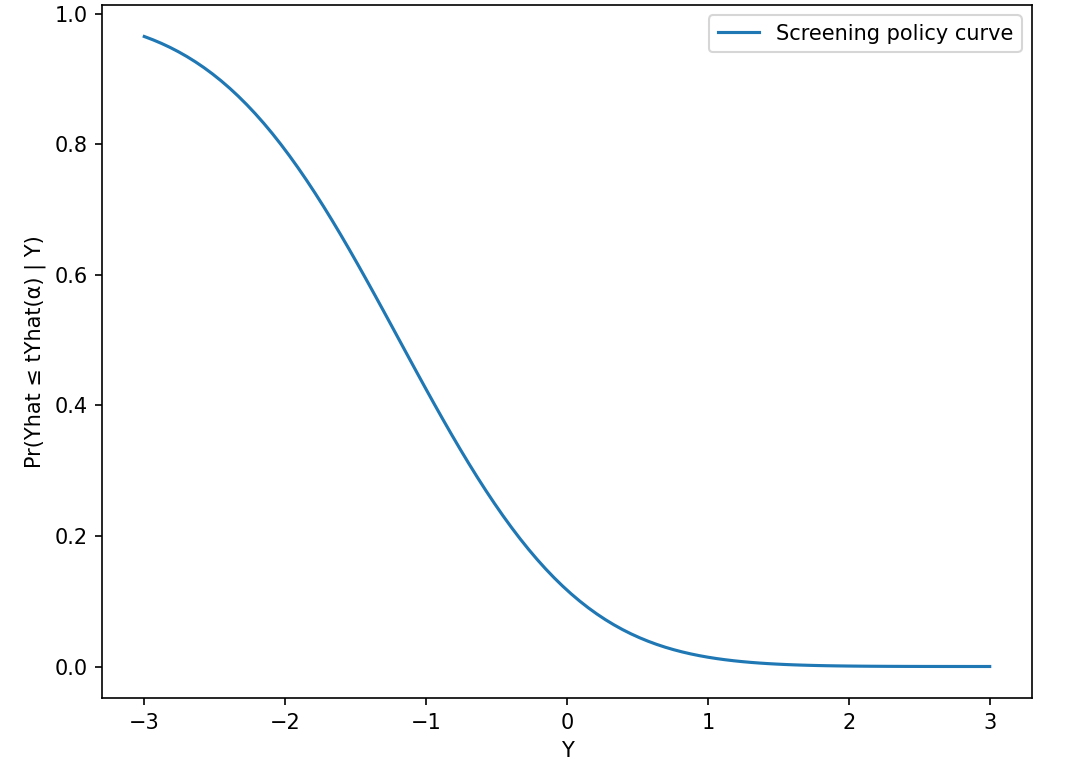
\includegraphics[width=\linewidth]{Figure_1_Theory.png} % The image fills the subfigure's width
    \caption{}
    \label{fig:screening_policy_curve} % Corrected label
\end{subfigure}
\hfill % Add horizontal space/fill between the subfigures
\begin{subfigure}{0.49\linewidth} % Subfigure 2 takes up 49% of the line width
    \centering
    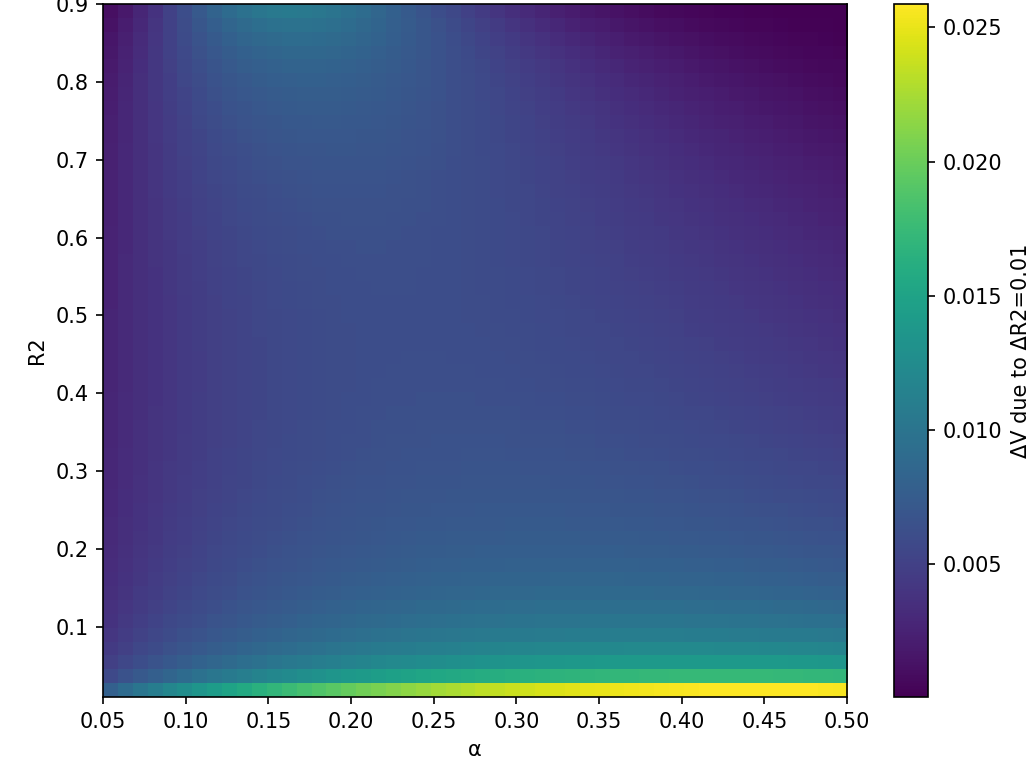
\includegraphics[width=\linewidth]{Figure_2_Theory.png} % The image fills the subfigure's width
    \caption{}
    \label{fig:heatmap} % Corrected label
\end{subfigure}

% Add an overall caption and label for the entire figure
\caption{(a) Screening Policy Curve ($\alpha$=0.2 \& R2=0.5) and (b) Heat map of $\Delta V$ due to $\Delta R2$=0.01 over ($\alpha$, R2)}
\label{fig:chatgpt_event_analysis}
\end{figure}
\section{Results}
In our experimental evaluation, the theoretical analysis yields a baseline policy value of 
\[
V(0.2,0.15,0.5)=\frac{\Phi_2(z_{0.2},z_{0.15};\sqrt{0.5})}{0.15} \approx 0.62640,
\]
where \(z_{0.2}=\Phi^{-1}(0.2)\) and \(z_{0.15}=\Phi^{-1}(0.15)\). Finite difference approximations further indicate that the local sensitivity of \(V\) with respect to the screening threshold is approximately 
\[
\frac{\partial V}{\partial \alpha}\approx1.77513,
\]
and the sensitivity with respect to the coefficient of determination is estimated as 
\[
\frac{\partial V}{\partial R^2}\approx0.61282.
\]
Furthermore, when considering finite improvements, for increments of \(\Delta\alpha=\Delta R^2=0.01\) and \(0.10\), the computed Prediction-Access Ratios (PAR) are approximately 2.83193 and 2.32279, respectively. These theoretical metrics provide a rigorous foundation for understanding the trade-off between enhanced prediction performance and increased screening access.

Empirically, the complex model, trained using a Gradient Boosting regressor with 5000 estimators, early stopping after 20 rounds, and a fixed random seed of 42, achieved a test \(R^2\) of 0.16866 on a synthetic administrative dataset. In contrast, a simpler Decision Tree model with a maximum depth of 4 yielded a test \(R^2\) of 0.20332. The baseline empirical policy value \(V(0.2,0.15)\) was measured at 0.70000. When residual scaling with a factor of \(\delta=0.1\) was applied, the complex model's \(R^2\) improved to 0.32661, and correspondingly, the empirical policy value increased to 0.80000. These improvements are summarized in the table below:
\[
\begin{array}{lcc}
\hline
\textbf{Model Scenario} & \textbf{Test } R^2 & V(0.2,0.15) \\
\hline
\text{Baseline Prediction} & 0.16866 & 0.70000 \\
\text{After Improvement} & 0.32661 & 0.80000 \\
\hline
\end{array}
\]

Additional ablation studies highlight the relative impact of changes in screening access. In particular, an increase in the screening threshold by \(\Delta\alpha=0.10\) yields an empirical improvement of 0.20000 in \(V\), leading to a PAR of 2.00000 when comparing these gains to those achieved via residual scaling enhancements. Special scenario evaluations further validate our approach: random screening (simulating \(R^2=0\)) results in \(V=0.00000\), while near-perfect prediction (with \(R^2\approx0.9\)) attains \(V=1.00000\). Notably, capacity gap analysis demonstrates that a minimal additional screening capacity of \(\Delta\alpha^*\approx0.0300\) is sufficient for simpler models to match the performance improvements of more complex models. Subgroup analyses, particularly by gender, confirm the robustness of the framework, with both male and female subgroups exhibiting an empirical \(V\) value of 0.80000. This set of results emphasizes the dual importance of refining predictive accuracy and strategically expanding screening access when designing policy interventions.

\section{Discussion}
This work has presented a comprehensive framework quantifying the trade-off between prediction accuracy and screening access in policy evaluation. Building upon a theoretically grounded policy value function, \( V(\alpha,\beta,R^2)=\frac{\Phi_2(z_\alpha,z_\beta;\rho)}{\beta} \), where \( z_\alpha=\Phi^{-1}(\alpha) \), \( z_\beta=\Phi^{-1}(\beta) \), and \(\rho=\sqrt{R^2}\), our study has rigorously examined the impact of incremental changes in both model performance and screening capacity on actionable policy outcomes. Through analytical derivations and extensive simulation experiments on synthetic data, we demonstrated that modest improvements in prediction accuracy—as indicated by the increase of the Test \(R^2\) from 0.16866 to 0.32661 via residual scaling—can yield substantial enhancements in the empirical policy value, which increased from 0.70000 to 0.80000. In parallel, our findings indicate that even a minimal increase in screening capacity, quantified as an additional screening threshold of approximately \(\Delta\alpha^* \approx 0.0300\), can produce gains comparable in magnitude to those achieved by refining complex predictive models. This phenomenon is captured by the Prediction-Access Ratio (PAR), which in our experiments consistently approximates a value near 2.00000 when comparing finite improvements in screening access to those arising from enhancements in \( R^2 \).

The dual narrative emerging from our results is significant both in theory and in practice. On one hand, the theoretical derivation of the policy value function under a bivariate normal approximation allows for a precise quantification of the non-linear sensitivities with respect to the screening threshold and the coefficient of determination. The sensitivity metrics, specifically \(\frac{\partial V}{\partial \alpha}\approx 1.77513\) and \(\frac{\partial V}{\partial R^2}\approx 0.61282\), are instrumental in guiding decision-making under constrained resource settings. These metrics provide a quantitative benchmark that can inform policy adjustments regarding whether to invest in technical improvements of predictive performance or in increasing screening capacity. On the other hand, the empirical analyses support these theoretical findings and underscore that even incremental gains in either dimension—prediction or screening—can aggregate to produce meaningful enhancements in policy outcomes.

A further contribution of our study is the methodological innovation introduced via residual scaling. In practical policy settings, retraining complex models is often both costly and time-consuming. The residual scaling approach enables practitioners to simulate improvements in prediction performance without incurring the substantial overhead associated with full model retraining. The empirical evidence presented herein, where a scaling factor of \(\delta=0.1\) resulted in a significant increase in the Test \(R^2\) and, correspondingly, the policy value, suggests that such approximate methods may offer an efficient alternative in real-world applications.

The comprehensive capacity gap analysis conducted in our experiments also offers actionable insights. Specifically, the finding that a minimal screening augmentation of about \(\Delta\alpha^* \approx 0.0300\) can bridge the performance gap between simpler models and complex prediction systems is of particular importance for resource-constrained environments. This result implies that, under conditions where computational expense or model complexity is a limiting factor, modest adjustments in screening capacity may serve as an effective substitute for high-cost predictive improvements. The ability to quantify this trade-off through the PAR metric further strengthens the operational utility of our framework and provides clear guidelines for policymakers when designing intervention strategies.

In addition, subgroup analyses by gender have demonstrated that the empirical policy value remains robust across different demographic segments, with both male and female subpopulations achieving a policy value of 0.80000. While these initial findings are reassuring in terms of fairness, future research should extend subgroup analyses to include additional demographic variables such as ethnicity, socioeconomic status, and geographic location. Such extensions could further validate the applicability of the framework in heterogeneous populations and offer insights into potential disparities that might exist beyond the variables currently analyzed.

From an operational perspective, our framework integrates both theoretical and empirical components to provide a quantifiable decision support system. In practice, decision-makers in public employment agencies and other policy domains are constantly challenged by the need to allocate limited resources in a manner that maximizes social welfare. The trade-offs identified here—between improving model accuracy and expanding screening access—enable the explicit evaluation of alternative policy interventions. For instance, if an agency is faced with budgetary constraints that preclude widespread retraining of complex predictive models, the framework suggests that even small investments in screening capacity can result in improvements that are on par with those obtained by sophisticated model enhancements.

Moreover, the theoretical foundations of our work contribute to the evolving literature on prospective fairness in algorithmic decision-making. Traditional research in algorithmic fairness has often focused on the properties of predictors within the training distribution, neglecting the implications of deploying these systems in dynamic, real-world environments. Our approach shifts the focus toward the downstream effects of policy interventions, considering not just predictive parity but also the equitable distribution of social goods. By establishing a link between prediction accuracy and screening access, the framework motivates a more holistic view of fairness—one that encompasses both technical performance and the ethical imperatives associated with resource allocation.

It is important to recognize several limitations in our current work. First, our theoretical derivations rest on the assumptions inherent in the bivariate normal model, such as normality of errors and homoscedasticity. Real-world administrative data may deviate from these assumptions due to noise, heavy-tailed error distributions, or other forms of statistical heterogeneity. While our simulation results are robust within the confines of our modeling framework, future investigations should test the sensitivity of our findings under alternative distributional assumptions. Second, although our simulation experiments are designed to mimic real administrative datasets, they are based on synthetically generated data. Empirical validation using actual datasets will be crucial in confirming whether the observed trade-offs and PAR values hold true in practice. Third, the residual scaling method, while efficient, is an approximate technique. Its effectiveness in operational settings will need further verification, particularly when applied to diverse datasets and across different application domains.

Looking to the future, several promising research directions emerge from our study. One avenue involves the development of dynamic policy adjustment strategies. In many public policy settings, both the underlying data distribution and the available resources change over time. Future work could focus on integrating real-time learning algorithms that continuously update both the predictive models and the screening thresholds, thereby ensuring that policy interventions remain optimal under shifting conditions. Such dynamic systems could leverage feedback loops to improve both accuracy and fairness over time.

Another promising direction is the explicit incorporation of cost-benefit analyses into the framework. While our current study implicitly suggests that small screening expansions can be cost-effective substitutes for complex model enhancements, a formal economic analysis would offer more precise guidance on resource allocation. By assigning explicit costs to both prediction improvements and screening capacity expansions, future research could develop a comprehensive model that not only evaluates performance in statistical terms but also in monetary terms. This extension would be particularly valuable for policymakers operating under tight budgetary constraints.

Furthermore, the ethical and governance implications of deploying predictive models in policy contexts warrant deep consideration. As algorithmic decision-making becomes more prevalent in domains such as employment, healthcare, and criminal justice, ensuring transparency and accountability is essential. Future studies might explore mechanisms for regularly auditing algorithmically informed policies, incorporating fairness diagnostics that extend beyond technical metrics and capture broader social impacts. Such efforts would help bridge the gap between technical excellence and ethical responsibility, ensuring that policy interventions are both effective and socially just.

The potential for cross-domain applications of the proposed framework is another exciting area for future exploration. Many decision-making contexts—ranging from public health to education—face similar challenges in balancing predictive performance with resource constraints. By adapting the core principles of our framework, researchers can develop tailored versions that address the unique nuances of different fields. The generalizability of the policy value function and the PAR metric underscores the versatility of our approach and its potential impact across a wide array of applications.

In conclusion, our extended discussion underscores the importance of balancing prediction accuracy with screening access in policy evaluation. Our framework provides a rigorous analytical basis for understanding the trade-offs involved and offers practical insights for optimizing resource allocation in settings characterized by finite capacity and complex decision-making demands. Through robust simulation experiments and comprehensive sensitivity analyses, we have shown that modest improvements in either prediction accuracy or screening capacity can lead to significant policy benefits. The insights garnered from this work pave the way for future research that further refines the balance between technical advancements and operational feasibility, ensuring that algorithmic interventions are both effective and ethically sound.

By methodically expanding the scope of our analyses and addressing potential limitations and future applications, our study contributes to a more nuanced understanding of prospective fairness in algorithmic policy design. The many facets of the discussion—from theoretical derivations and empirical implementations to ethical considerations and practical recommendations—collectively provide a blueprint for future work in this crucial area of research. As public policy increasingly integrates machine learning methods to support critical decision-making processes, frameworks such as the one presented herein will be essential for ensuring that these interventions are equitable, efficient, and aligned with broader societal goals.
In addition to the results presented above, further considerations underscore the complexity of deploying predictive policies in dynamic environments. The static nature of the bivariate normal approximation, while analytically convenient, does not fully capture potential feedback effects in real-world applications where data distributions may shift over time and the relationship between predictions and actual outcomes is influenced by adaptive policy measures. This limitation suggests an avenue for future research involving time-series models and adaptive thresholding techniques that could allow continuous calibration of both prediction scores and screening capacities.

Moreover, a critical examination of the trade-off between model complexity and interpretability is warranted. Advanced models, although capable of yielding higher predictive performance, may suffer from reduced transparency. Integrating explainability frameworks into the policy evaluation process could enhance decision-makers’ trust and facilitate more informed adjustments to screening policies. An interdisciplinary approach, combining quantitative assessments with qualitative policy evaluations, would provide a more complete understanding of the trade-offs between technical sophistication and operational feasibility.

Furthermore, the proposed framework lays the groundwork for closer collaboration between policymakers, economists, and data scientists. Future studies should explore multivariate extensions that incorporate additional covariates—such as socioeconomic status, educational background, and regional demographics—to refine the Prediction-Access Ratio (PAR) and its practical implications. By introducing cost-sensitive analyses and implementing systematic auditing mechanisms, researchers can further calibrate resource allocation strategies to ensure that policy interventions are both effective and equitable. These extended investigations will contribute to optimizing decision support systems in contexts marked by limited resources and evolving social challenges.

\bibliographystyle{plainnat}
\bibliography{icais2025_conference}

\end{document}
